% Many modern multi-talker Automatic Speech Recognition (ASR) systems require world-level timing information for training. In token-level Serialized Output Training \cite{kanda22_interspeech} (t-SOT) timing is required for constructing the training targets in the correct order; the Diarization Conditioned Whisper (DiCoW) model family \cite{polok2026dicow} requires time stamps to prepare supervisions for the 30s audio chunks used for fine-tuning Whisper, which it re-purposes for multi-talker ASR.

% Unfortunately, obtaining time-stamped transcripts is difficult. World-level time-stamps in common multi-talker ASR corpora, such as AMI \cite{carletta2005ami}, and NOTSOFAR-1 (NSF1) \cite{vinnikov2024notsofar}, are possible thanks to an expensive data collection procedures involving separate close-talk, or throat microphones. These speaker-specific channels enable the use of well-established forced alignment methods \cite{mcauliffe2017montreal} to retrieve time-stamped transcripts. Some corpora are even manually annotated for timing information \cite{pitt2005buckeye, garofolo1993timit}.

% Standard forced alignment relies on Viterbi search through a transcript graph in which each transition represents the time at which a label is produced. However, this procedure does not scale well to long recordings. Common approaches \cite{katsamanis2011sailalign, checkpointing, CTC_align, mcauliffe2017montreal} for long-form alignment, such as \textsc{Sail}, \textsc{CTC align}, or \textsc{kaldi}-based recipes \cite{povey2011kaldi}, use an initial step of voice activity detection (VAD) or first-pass decoding (possibly transcript-biased decoding \cite{biased_LMs}) to create more manageable segments. However, this approach struggles in multi-talker scenarios as continuous conversation means there are few regions of silence since at least one person is usually speaking. Forced alignment is also not well equipped to deal with overlapped speech, and forced alignment packages, such as the Montreal Forced Aligner (MFA), do not work well in this scenario. Even when speech can be aligned, it is not very useful without speaker attribution (see Fig. \ref{fig:overlapped_attribution}).
% %e.g., A: How old are you? B: twenty C: eight, has a very different meaning from, A: How old are you? B: twenty-eight, or A: How old are you? twenty-eight?

% We recently proposed using alignment graphs constructed from the shuffle product of multi-talker transcripts \cite{wiesner2026modeling}, and showed some promising preliminary results on synthetic 2 and 3 speaker 30\,s audio clips. However, the method, at least when applied naively, does not scale to longer audio recordings or to more speakers, making it unsuitable for alignment of long-form conversational speech such as meeting scenarios~\cite{carletta2005ami, vinnikov2024notsofar, cornell2025recent}. Furthermore, in multi-talker forced alignment, localizing a token (phoneme, byte-pair encoding-unit, word, or syllable) in time only partially solves the alignment problem as also speaker attribution is essential. In \cite{wiesner2026modeling} we did not  explore this problem or to what extent alignment is possible without speaker attributed transcripts.

% \begin{figure}[t]
\centering
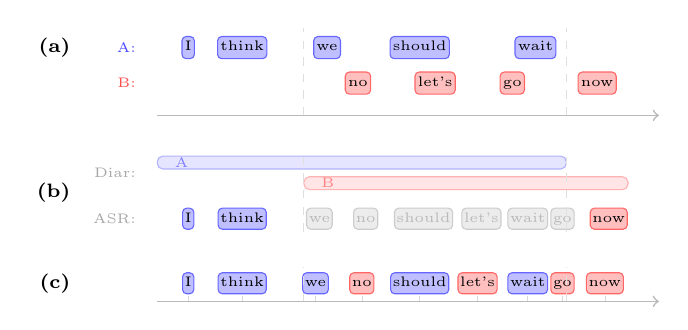
\begin{tikzpicture}[
    xscale=0.98,
    yscale=0.82,
    spkA/.style={fill=blue!25, draw=blue!60, rounded corners=1.5pt, minimum height=0.28cm, inner sep=1pt, font=\tiny\strut},
    spkB/.style={fill=red!25, draw=red!60, rounded corners=1.5pt, minimum height=0.28cm, inner sep=1pt, font=\tiny\strut},
    spkAt/.style={fill=blue!25, draw=blue!60, rounded corners=1.5pt, minimum height=0.26cm, inner sep=0.8pt, font=\tiny\strut},
    spkBt/.style={fill=red!25, draw=red!60, rounded corners=1.5pt, minimum height=0.26cm, inner sep=0.8pt, font=\tiny\strut},
    amb/.style={fill=gray!15, draw=gray!40, rounded corners=1.5pt, minimum height=0.24cm, inner sep=0.8pt, font=\tiny\strut, text=gray!55},
    timeline/.style={->, semithick, gray!55},
    lbl/.style={font=\scriptsize\bfseries, anchor=east},
]

% ---- (a) Ground truth ----
\node[lbl] at (-0.7, 2.6) {(a)};

\node[spkA] at (0.7, 2.6) {I};
\node[spkA] at (1.4, 2.6) {think};
\node[spkA] at (2.5, 2.6) {we};
\node[spkA] at (3.7, 2.6) {should};
\node[spkA] at (5.2, 2.6) {wait};

\node[spkB] at (2.9, 2.05) {no};
\node[spkB] at (3.9, 2.05) {let's};
\node[spkB] at (4.9, 2.05) {go};
\node[spkB] at (6.0, 2.05) {now};

\node[font=\tiny, blue!70, anchor=east] at (0.15, 2.6) {A:};
\node[font=\tiny, red!70, anchor=east] at (0.15, 2.05) {B:};

\draw[timeline] (0.3, 1.55) -- (6.8, 1.55);
\draw[dashed, gray!25, thin] (2.2, 1.55) -- (2.2, 2.9);
\draw[dashed, gray!25, thin] (5.6, 1.55) -- (5.6, 2.9);


% ---- (b) Cascade ----
\node[lbl] at (-0.7, 0.35) {(b)};

\draw[fill=blue!10, draw=blue!30, rounded corners=2pt] (0.3, 0.72) rectangle (5.6, 0.92);
\node[font=\tiny, blue!50, anchor=west] at (0.4, 0.82) {A};
\draw[fill=red!10, draw=red!30, rounded corners=2pt] (2.2, 0.4) rectangle (6.4, 0.6);
\node[font=\tiny, red!50, anchor=west] at (2.3, 0.5) {B};
\node[font=\tiny, gray!70, anchor=east] at (0.15, 0.66) {Diar:};

\node[font=\tiny, gray!70, anchor=east] at (0.15, -0.05) {ASR:};
\node[spkAt] at (0.7, -0.05) {I};
\node[spkAt] at (1.4, -0.05) {think};
\node[amb] at (2.4, -0.05) {we};
\node[amb] at (3.0, -0.05) {no};
\node[amb] at (3.75, -0.05) {should};
\node[amb] at (4.5, -0.05) {let's};
\node[amb] at (5.1, -0.05) {wait};
\node[amb] at (5.55, -0.05) {go};
\node[spkBt] at (6.15, -0.05) {now};

\draw[dashed, gray!25, thin] (2.2, -0.25) -- (2.2, 1.0);
\draw[dashed, gray!25, thin] (5.6, -0.25) -- (5.6, 1.0);


% ---- (c) Shuffle ----
\node[lbl] at (-0.7, -1.05) {(c)};

\node[spkAt] at (0.7, -1.05) {I};
\node[spkAt] at (1.4, -1.05) {think};
\node[spkAt] at (2.35, -1.05) {we};
\node[spkBt] at (2.95, -1.05) {no};
\node[spkAt] at (3.7, -1.05) {should};
\node[spkBt] at (4.45, -1.05) {let's};
\node[spkAt] at (5.1, -1.05) {wait};
\node[spkBt] at (5.55, -1.05) {go};
\node[spkBt] at (6.1, -1.05) {now};

\foreach \x in {0.7, 1.4, 2.35, 2.95, 3.7, 4.45, 5.1, 5.55, 6.1} {
    \draw[gray!30, very thin] (\x, -1.25) -- (\x, -1.33);
}
\draw[timeline] (0.3, -1.33) -- (6.8, -1.33);

\draw[dashed, gray!25, thin] (2.2, -1.33) -- (2.2, -0.8);
\draw[dashed, gray!25, thin] (5.6, -1.33) -- (5.6, -0.8);

\end{tikzpicture}
\caption{%
Word-level speaker attribution in overlapped speech.
\textbf{(a)}~Ground truth: speakers A (\textcolor{blue!60}{blue}) and B (\textcolor{red!60}{red}) produce concurrent tokens with partial overlap (dashed).
\textbf{(b)}~Cascade: diarization detects both speakers as active, but all ASR words in the overlap are ambiguous (gray) since both segments cover the same time.
\textbf{(c)}~Shuffle: the Viterbi path produces an interleaved, time-aligned, speaker-attributed sequence.
}
\label{fig:overlapped_attribution}
\vspace{-4mm}
\end{figure}

% Speaker diariazation, i.e., ``who spoke when,'' partially solves this task.
% %However, multi-talker alignment deals with speaker attribution of labels, not frames. In non-overlapped speech, these are equivalent problems -- one can decode each speaker specific segment and trivially assign all decoded tokens to the speaker of that segment. 
% %Conversely, if one can decode a single-speaker segment of speech and assign the decoded tokens to a speaker, e.g., by using a language model (LM) to detect switch points, then the speech is effectively diarized.
% In overlapped speech, however, frame-level activity does not uniquely determine the attribution of linguistic events and can result in combinatorially many ways of attributing tokens to speakers. 
% % Recent work addressing this problem has used serialized output training (SOT)~\cite{}, or iterative target speaker decoding to handle overlapped speech. However, these approaches often rely on a separate diarization system and do not easily support fine-grained alignment similar to traditional Viterbi-based alignment in HMM-GMM, CTC, or Transducer models.  
% % Furthermore, the most egregious ASR errors in multi-talker ASR come from assigning recognized output to the wrong speaker. In the case of cpWER~\cite{}, for example, the mis-attributed tokens count both as insertions with respect to the wrongly hypothesized speaker, and also as deletions with respect to the missed reference speaker, even if the hypothesized transcript is correct. Fixing such errors has the potential to dramatically improve multi-talker ASR performance.
% We therefore treat diarization as the task of assigning speakers to temporally localized labels. This directly answers the question ``who produced which label'' and since each label can still be approximately mapped to frame-level activity, it also solves the problem of ``who spoke when.'' Furthermore, our approach enables transcript conditioned diarization via alignment of audio to a set of transcripts. We therefore shift the problem from frame-level diarization to label synchronous diarization by modeling overlapped speech using shuffles as in \cite{wiesner2026modeling}, whose formulation unifies the treatment of overlapped and non-overlapped speech and enables one-pass multi-talker forced alignment. We demonstrate our approach on the AMI \cite{} and NOTSOFAR \cite{} datasets. %We also show the speaker attribution performance in terms of word diarization error rate (WDER) and diarization error rate of the speaker attribution component of the shuffle models, which has not been previously explored. The 
%---------------------
% Many multi-talker automatic speech recognition (ASR) systems require word-level timing information for training. In token-level serialized output training (t-SOT)~\cite{kanda22_interspeech} timing is required to construct the training targets in the correct order; the diarization-conditioned Whisper (DiCoW) family~\cite{polok2026dicow} requires timestamps to prepare supervisions for the 30\,s chunks used to fine-tune Whisper for multi-talker ASR. Obtaining such transcripts is difficult. Word-level timestamps in corpora such as AMI~\cite{carletta2005ami} and NOTSOFAR-1 (NSF1)~\cite{vinnikov2024notsofar} exist only because each speaker was recorded on a separate close-talk or throat microphone, to which well-established single-speaker forced alignment~\cite{mcauliffe2017montreal} can be applied. Most multi-talker audio has a transcript but no per-speaker channel, and, to our knowledge, no single technique produces speaker-attributed word timing from the mixture alone. 
% Some large-scale text-to-speech data pipelines~\cite{he2024emilia, jung2026sommelier} instead apply source separation and diarization to obtain single-speaker segments that a standard aligner can process. This is effective on web audio with limited overlap, but in far-field conversational scenatios neural speech separation degrades and ceases to be effective, in particular as a front-end for ASR~\cite{cornell2025recent}. 

% Forced alignment of single-speaker audio is a well-established problem. HMM-based aligners such as MFA~\cite{mcauliffe2017montreal, povey2011kaldi}, CTC-based aligners~\cite{huang2024less, rastorgueva2023nfa, bain2023whisperx} and recent saliency-based approaches~\cite{zeyer2026gradient} all model one token sequence and one active speaker per frame. Since Viterbi search through a transcript graph does not scale to long recordings, they segment the audio with voice activity detection (VAD) or a first decoding pass, possibly biased towards the transcript ~\cite{lamel2002lightly, manohar2017jhu}, and align each segment separately~\cite{moreno1998recursive, katsamanis2011sailalign}. This strategy requires either silent regions at which to segment or a first pass that is accurate enough to provide anchors. The alternative is to keep the exact search and reduce its memory, for instance by check-pointing the Viterbi algorithm~\cite{grice1997reduced} or by pruning it to a band~\cite{kuang2022pruned}. 
% Moreover, even when close-talk microphones exist, overlapped speech remains an obstacle. On mixed-headset AMI recordings, MFA produced an alignment for only 5 of 16 meetings~\cite{rastorgueva2023nfa}, and the aligners that succeeded did so on a transcript in which all speakers' words were concatenated into a single sequence. Their output therefore carries no speaker attribution, which most applications require: localizing a token (phoneme, byte-pair unit, word or syllable) in time solves only part of the multi-talker alignment problem (Fig.~\ref{fig:overlapped_attribution}).

% \begin{figure}[t]
\centering
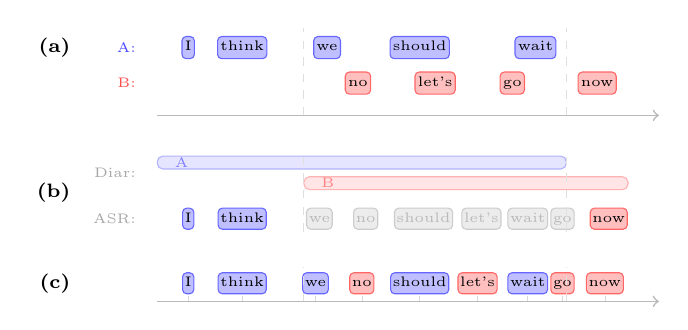
\begin{tikzpicture}[
    xscale=0.98,
    yscale=0.82,
    spkA/.style={fill=blue!25, draw=blue!60, rounded corners=1.5pt, minimum height=0.28cm, inner sep=1pt, font=\tiny\strut},
    spkB/.style={fill=red!25, draw=red!60, rounded corners=1.5pt, minimum height=0.28cm, inner sep=1pt, font=\tiny\strut},
    spkAt/.style={fill=blue!25, draw=blue!60, rounded corners=1.5pt, minimum height=0.26cm, inner sep=0.8pt, font=\tiny\strut},
    spkBt/.style={fill=red!25, draw=red!60, rounded corners=1.5pt, minimum height=0.26cm, inner sep=0.8pt, font=\tiny\strut},
    amb/.style={fill=gray!15, draw=gray!40, rounded corners=1.5pt, minimum height=0.24cm, inner sep=0.8pt, font=\tiny\strut, text=gray!55},
    timeline/.style={->, semithick, gray!55},
    lbl/.style={font=\scriptsize\bfseries, anchor=east},
]

% ---- (a) Ground truth ----
\node[lbl] at (-0.7, 2.6) {(a)};

\node[spkA] at (0.7, 2.6) {I};
\node[spkA] at (1.4, 2.6) {think};
\node[spkA] at (2.5, 2.6) {we};
\node[spkA] at (3.7, 2.6) {should};
\node[spkA] at (5.2, 2.6) {wait};

\node[spkB] at (2.9, 2.05) {no};
\node[spkB] at (3.9, 2.05) {let's};
\node[spkB] at (4.9, 2.05) {go};
\node[spkB] at (6.0, 2.05) {now};

\node[font=\tiny, blue!70, anchor=east] at (0.15, 2.6) {A:};
\node[font=\tiny, red!70, anchor=east] at (0.15, 2.05) {B:};

\draw[timeline] (0.3, 1.55) -- (6.8, 1.55);
\draw[dashed, gray!25, thin] (2.2, 1.55) -- (2.2, 2.9);
\draw[dashed, gray!25, thin] (5.6, 1.55) -- (5.6, 2.9);


% ---- (b) Cascade ----
\node[lbl] at (-0.7, 0.35) {(b)};

\draw[fill=blue!10, draw=blue!30, rounded corners=2pt] (0.3, 0.72) rectangle (5.6, 0.92);
\node[font=\tiny, blue!50, anchor=west] at (0.4, 0.82) {A};
\draw[fill=red!10, draw=red!30, rounded corners=2pt] (2.2, 0.4) rectangle (6.4, 0.6);
\node[font=\tiny, red!50, anchor=west] at (2.3, 0.5) {B};
\node[font=\tiny, gray!70, anchor=east] at (0.15, 0.66) {Diar:};

\node[font=\tiny, gray!70, anchor=east] at (0.15, -0.05) {ASR:};
\node[spkAt] at (0.7, -0.05) {I};
\node[spkAt] at (1.4, -0.05) {think};
\node[amb] at (2.4, -0.05) {we};
\node[amb] at (3.0, -0.05) {no};
\node[amb] at (3.75, -0.05) {should};
\node[amb] at (4.5, -0.05) {let's};
\node[amb] at (5.1, -0.05) {wait};
\node[amb] at (5.55, -0.05) {go};
\node[spkBt] at (6.15, -0.05) {now};

\draw[dashed, gray!25, thin] (2.2, -0.25) -- (2.2, 1.0);
\draw[dashed, gray!25, thin] (5.6, -0.25) -- (5.6, 1.0);


% ---- (c) Shuffle ----
\node[lbl] at (-0.7, -1.05) {(c)};

\node[spkAt] at (0.7, -1.05) {I};
\node[spkAt] at (1.4, -1.05) {think};
\node[spkAt] at (2.35, -1.05) {we};
\node[spkBt] at (2.95, -1.05) {no};
\node[spkAt] at (3.7, -1.05) {should};
\node[spkBt] at (4.45, -1.05) {let's};
\node[spkAt] at (5.1, -1.05) {wait};
\node[spkBt] at (5.55, -1.05) {go};
\node[spkBt] at (6.1, -1.05) {now};

\foreach \x in {0.7, 1.4, 2.35, 2.95, 3.7, 4.45, 5.1, 5.55, 6.1} {
    \draw[gray!30, very thin] (\x, -1.25) -- (\x, -1.33);
}
\draw[timeline] (0.3, -1.33) -- (6.8, -1.33);

\draw[dashed, gray!25, thin] (2.2, -1.33) -- (2.2, -0.8);
\draw[dashed, gray!25, thin] (5.6, -1.33) -- (5.6, -0.8);

\end{tikzpicture}
\caption{%
Word-level speaker attribution in overlapped speech.
\textbf{(a)}~Ground truth: speakers A (\textcolor{blue!60}{blue}) and B (\textcolor{red!60}{red}) produce concurrent tokens with partial overlap (dashed).
\textbf{(b)}~Cascade: diarization detects both speakers as active, but all ASR words in the overlap are ambiguous (gray) since both segments cover the same time.
\textbf{(c)}~Shuffle: the Viterbi path produces an interleaved, time-aligned, speaker-attributed sequence.
}
\label{fig:overlapped_attribution}
\vspace{-4mm}
\end{figure}

% In~\cite{wiesner2026modeling} we recently proposed constructing alignment graphs from the shuffle product of multi-talker transcripts. The shuffle formulation treats overlapped and non-overlapped speech uniformly and permits multi-talker forced alignment in a single Viterbi pass, and we reported results on synthetic 30\,s mixtures of two and three speakers. That work has however two limitations that this paper addresses. First, applied without modification, the method does not scale to longer recordings or to more speakers, and cannot be used on long-form conversational speech such as meetings~\cite{carletta2005ami, vinnikov2024notsofar, cornell2025recent}. Second, it assumed speaker-attributed transcripts, whereas in practice transcripts often carry utterance boundaries but no speaker labels. Speaker diarization, which determines who spoke when, does not resolve this case: in overlapped speech, frame-level activity does not determine which speaker produced which token, and the number of consistent assignments grows combinatorially. Attributing utterances to speakers is an instance of the speaker partitioning problem of Br\"ummer and de Villiers~\cite{brummer2010speaker}, whose solution space grows with the Bell numbers and which clustering methods such as VBx~\cite{landini2022bayesian} solve approximately from acoustics alone. We instead treat diarization as the assignment of speakers to temporally localized labels, which specifies which speaker produced each label and, since each label maps to a set of frames, also who spoke when. This label-synchronous view permits transcript-conditioned diarization: the audio is aligned to a set of transcripts without speaker labels, and the speaker partition is then scored under the acoustic model given the token alignment.

% The contributions of this paper are: (i) a set of inference techniques that make shuffle-based alignment of long recordings with many speakers feasible on a single GPU, each evaluated in an ablation (Section~\ref{sec:longform}); (ii) a method for speaker attribution of transcripts without speaker labels, formulated as token alignment followed by a search over speaker partitions using the frame-level speaker posteriors of a speaker-attributed shuffle model (Section~\ref{sec:attribution}); and (iii) an out-of-domain evaluation on AMI and NSF1 of models trained only on synthetic and web-scraped data, which are publicly released.
%----------------------------
Many multi-talker automatic speech recognition (ASR) systems require word-level timing information for training. Token-level serialized output training (t-SOT)~\cite{kanda22_interspeech} uses timing to order training targets, while diarization-conditioned Whisper (DiCoW)~\cite{polok2026dicow} requires timestamps to prepare supervision for the 30\,s chunks used to fine-tune Whisper. Word-level timestamps are difficult to obtain. In corpora such as AMI~\cite{carletta2005ami} and NOTSOFAR-1 (NSF)~\cite{vinnikov2024notsofar} they exist because a separate close-talk or throat microphone recorded each speaker, enabling single-speaker forced alignment~\cite{mcauliffe2017montreal}. Most multi-talker recordings separate speaker channels and, to our knowledge, no single technique produces speaker-attributed word timing directly from the mixture. Large-scale text-to-speech pipelines~\cite{he2024emilia, jung2026sommelier} cascade source separation and diarization to obtain single-speaker segments for alignment, but separation degrades in far-field conversational speech, particularly as an ASR front end~\cite{cornell2025recent}.

Forced alignment of single-speaker audio is well established. HMM-based aligners such as MFA~\cite{mcauliffe2017montreal, povey2011kaldi}, connectionist temporal classification (CTC)-based aligners~\cite{huang2024less, rastorgueva2023nfa, bain2023whisperx},
and recent saliency-based approaches~\cite{zeyer2026gradient} assume one token sequence and one active speaker per frame. Because exact Viterbi search through long transcript graphs is memory intensive, long recordings are commonly segmented using VAD or a first decoding pass, possibly biased toward the transcript~\cite{ manohar2017jhu}, and aligned segment by segment~\cite{moreno1998recursive, katsamanis2011sailalign}. This requires either suitable silence boundaries or sufficiently accurate anchors. Alternatives retain the exact search while reducing memory, for example through Viterbi checkpointing~\cite{grice1997reduced} or band pruning~\cite{kuang2022pruned}. Overlap is problematic even with close-talk microphones: on mixed-headset AMI recordings, MFA aligned only 5 of 16 meetings~\cite{rastorgueva2023nfa}. Successful aligners operated on a single sequence formed by concatenating all speakers' words, but outputs then lack speaker attribution: localizing a token in time is only one part of multi-talker alignment (Figure ~\ref{fig:overlapped_attribution}).

\begin{figure}[t]
\centering
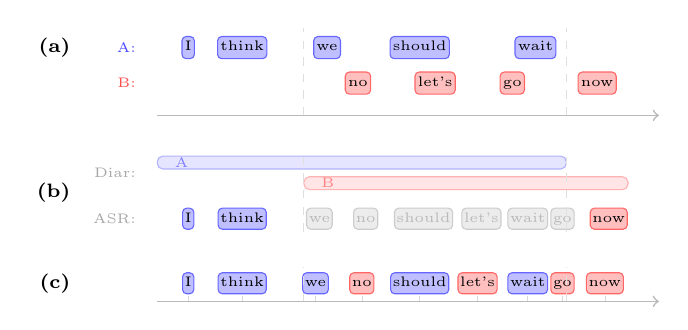
\begin{tikzpicture}[
    xscale=0.98,
    yscale=0.82,
    spkA/.style={fill=blue!25, draw=blue!60, rounded corners=1.5pt, minimum height=0.28cm, inner sep=1pt, font=\tiny\strut},
    spkB/.style={fill=red!25, draw=red!60, rounded corners=1.5pt, minimum height=0.28cm, inner sep=1pt, font=\tiny\strut},
    spkAt/.style={fill=blue!25, draw=blue!60, rounded corners=1.5pt, minimum height=0.26cm, inner sep=0.8pt, font=\tiny\strut},
    spkBt/.style={fill=red!25, draw=red!60, rounded corners=1.5pt, minimum height=0.26cm, inner sep=0.8pt, font=\tiny\strut},
    amb/.style={fill=gray!15, draw=gray!40, rounded corners=1.5pt, minimum height=0.24cm, inner sep=0.8pt, font=\tiny\strut, text=gray!55},
    timeline/.style={->, semithick, gray!55},
    lbl/.style={font=\scriptsize\bfseries, anchor=east},
]

% ---- (a) Ground truth ----
\node[lbl] at (-0.7, 2.6) {(a)};

\node[spkA] at (0.7, 2.6) {I};
\node[spkA] at (1.4, 2.6) {think};
\node[spkA] at (2.5, 2.6) {we};
\node[spkA] at (3.7, 2.6) {should};
\node[spkA] at (5.2, 2.6) {wait};

\node[spkB] at (2.9, 2.05) {no};
\node[spkB] at (3.9, 2.05) {let's};
\node[spkB] at (4.9, 2.05) {go};
\node[spkB] at (6.0, 2.05) {now};

\node[font=\tiny, blue!70, anchor=east] at (0.15, 2.6) {A:};
\node[font=\tiny, red!70, anchor=east] at (0.15, 2.05) {B:};

\draw[timeline] (0.3, 1.55) -- (6.8, 1.55);
\draw[dashed, gray!25, thin] (2.2, 1.55) -- (2.2, 2.9);
\draw[dashed, gray!25, thin] (5.6, 1.55) -- (5.6, 2.9);


% ---- (b) Cascade ----
\node[lbl] at (-0.7, 0.35) {(b)};

\draw[fill=blue!10, draw=blue!30, rounded corners=2pt] (0.3, 0.72) rectangle (5.6, 0.92);
\node[font=\tiny, blue!50, anchor=west] at (0.4, 0.82) {A};
\draw[fill=red!10, draw=red!30, rounded corners=2pt] (2.2, 0.4) rectangle (6.4, 0.6);
\node[font=\tiny, red!50, anchor=west] at (2.3, 0.5) {B};
\node[font=\tiny, gray!70, anchor=east] at (0.15, 0.66) {Diar:};

\node[font=\tiny, gray!70, anchor=east] at (0.15, -0.05) {ASR:};
\node[spkAt] at (0.7, -0.05) {I};
\node[spkAt] at (1.4, -0.05) {think};
\node[amb] at (2.4, -0.05) {we};
\node[amb] at (3.0, -0.05) {no};
\node[amb] at (3.75, -0.05) {should};
\node[amb] at (4.5, -0.05) {let's};
\node[amb] at (5.1, -0.05) {wait};
\node[amb] at (5.55, -0.05) {go};
\node[spkBt] at (6.15, -0.05) {now};

\draw[dashed, gray!25, thin] (2.2, -0.25) -- (2.2, 1.0);
\draw[dashed, gray!25, thin] (5.6, -0.25) -- (5.6, 1.0);


% ---- (c) Shuffle ----
\node[lbl] at (-0.7, -1.05) {(c)};

\node[spkAt] at (0.7, -1.05) {I};
\node[spkAt] at (1.4, -1.05) {think};
\node[spkAt] at (2.35, -1.05) {we};
\node[spkBt] at (2.95, -1.05) {no};
\node[spkAt] at (3.7, -1.05) {should};
\node[spkBt] at (4.45, -1.05) {let's};
\node[spkAt] at (5.1, -1.05) {wait};
\node[spkBt] at (5.55, -1.05) {go};
\node[spkBt] at (6.1, -1.05) {now};

\foreach \x in {0.7, 1.4, 2.35, 2.95, 3.7, 4.45, 5.1, 5.55, 6.1} {
    \draw[gray!30, very thin] (\x, -1.25) -- (\x, -1.33);
}
\draw[timeline] (0.3, -1.33) -- (6.8, -1.33);

\draw[dashed, gray!25, thin] (2.2, -1.33) -- (2.2, -0.8);
\draw[dashed, gray!25, thin] (5.6, -1.33) -- (5.6, -0.8);

\end{tikzpicture}
\caption{%
Word-level speaker attribution in overlapped speech.
\textbf{(a)}~Ground truth: speakers A (\textcolor{blue!60}{blue}) and B (\textcolor{red!60}{red}) produce concurrent tokens with partial overlap (dashed).
\textbf{(b)}~Cascade: diarization detects both speakers as active, but all ASR words in the overlap are ambiguous (gray) since both segments cover the same time.
\textbf{(c)}~Shuffle: the Viterbi path produces an interleaved, time-aligned, speaker-attributed sequence.
}
\label{fig:overlapped_attribution}
\vspace{-4mm}
\end{figure}

In~\cite{wiesner2026modeling} we proposed constructing alignment graphs from the shuffle product of multi-talker transcripts, treating overlapped and non-overlapped speech uniformly and enabling multi-talker forced alignment in a single Viterbi pass. We evaluated the approach on synthetic 30s mixtures of two and three speakers, but it has two limitations addressed here. First, without modification it does not easily scale to longer recordings or more speakers, preventing application to meeting-style speech~\cite{carletta2005ami, vinnikov2024notsofar, cornell2025recent}. Second, it assumes speaker-attributed transcripts, whereas practical transcripts often provide utterance boundaries but no speaker labels. Speaker diarization alone does not resolve this ambiguity in overlapped speech: frame-level activity does not uniquely determine who produced each token.

Assigning utterances to speakers is an instance of the speaker partitioning problem~\cite{brummer2010speaker}, whose solution space grows with the Bell numbers and which clustering methods such as VBx~\cite{landini2022bayesian} solve approximately from acoustics alone. Similar to \cite{9746225},  we instead view diarization as assigning temporally localized labels to speakers. This permits transcript-conditioned diarization, similar in spirit to \cite{shafey19_interspeech, park19_interspeech}: the audio is first aligned to transcripts without speaker labels, after which speaker partitions are scored under the acoustic model given the token alignment.

The contributions of this paper are: (i) inference techniques that make shuffle-based alignment of long recordings with many speakers feasible on a single GPU, evaluated by ablation (Section~\ref{sec:results_longform}); (ii) speaker attribution for transcripts without speaker labels, formulated as token alignment followed by search over speaker partitions using frame-level speaker posteriors from a speaker-attributed shuffle model (Section~\ref{sec:speaker_attribution}); and (iii) out-of-domain evaluation of publicly released models trained only on synthetic and web-scraped data on the AMI and NSF1 single distant microphone (SDM) condition.